\chapter{Verfahrensbeschreibung}\label{ch:verfahrensbeschreibung}


\section{Mathematischer Hintergrund}\label{sec:mathematischer_hintergrund}
Das System arbeitet verschiedenen mathematischen Verfahren mit welchen die benötigten Berechnungen durchgeführt werden.

\subsection{Formel von Heron}\label{subsec:formel_von_heron}
Zum berechnen des Flächeninhalts eines Dreiecks wird die Formel von Heron verwendet.
\\
Der Satz von Heron besagt, dass die Fläche eines Dreiecks durch die Länge seiner Seiten berechnet werden kann. Mathematisch ausgedrückt:

\begin{align}
    A=\sqrt{s(s-a)(s-b)(s-c)}\\
\end{align}
Wobei $s$ für die Hälfte des Umfangs steht:
\begin{align}
    s=\frac{a+b+c}{2}
\end{align}

\subsection{Satz des Pythagoras}\label{subsec:satz_des_pythagoras}
Zum überprüfen ob ein Dreieck rechtwinklig ist, wird der Satz des Pythagoras verwendet.
\\
Der Satz des Pythagoras besagt, dass in einem rechtwinkligen Dreieck die Summe der Kathetenquadrate gleich dem Hypothenusenquadrat ist. Mathematisch ausgedrückt:

\begin{align}
    a^2+b^2=c^2\\
\end{align}

Bildlich veranschaut sieht die Formel wie folgt aus:

\begin{figure}
    \centering
    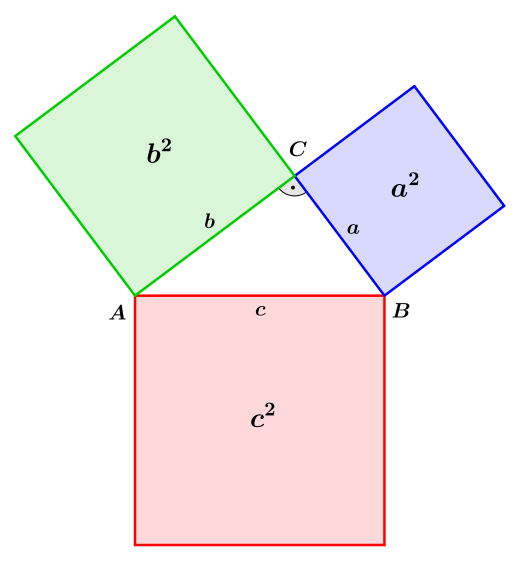
\includegraphics[width=0.5\textwidth]{images/pythagoras.png}
    \caption{Satz des Pythagoras}
    \label{fig:pythagoras}
\end{figure}
